% Background chapter continued..

\section{Similarity Methods}
\label{similarity_methods}
In this section several methods are discussed to calculate similarity score between two vectors.
\subsection{Cosine Similarity}
\label{cosine_similarity}

In cosine similarity measure \cite{19}, the result is the cosine of the angle between two vectors. It  discovers the direction between two vectors if it is same or not. Often, cosine similarity is used to calculate document similarity in text analysis. The item ratings or preferences are stored in one vector called as item vector. The preferences of user are stored in another vector based on user's ratings and likes-dislikes is known as profile vector. Consider $A = (5,0,3,0,2)$ and $B = (3,0,2,0,2)$ are profile vector and item vector respectively, then the similarity between them can be calculated as per \autoref{eq:cosine_similarity}.
\begin{equation}
sim(A,B) = \frac {A \cdot B}{\parallel A \parallel \parallel B \parallel} = \frac{\sum_{i=1}^{n} {A_{i} B_{i}}}{\sqrt{\sum_{i=1}^{n} {A_{i}^2}} \sqrt{\sum_{i=1}^{n} {B_{i}^2}}}
\label{eq:cosine_similarity}
\end{equation}
\begin{figure}[H]
	\centering
	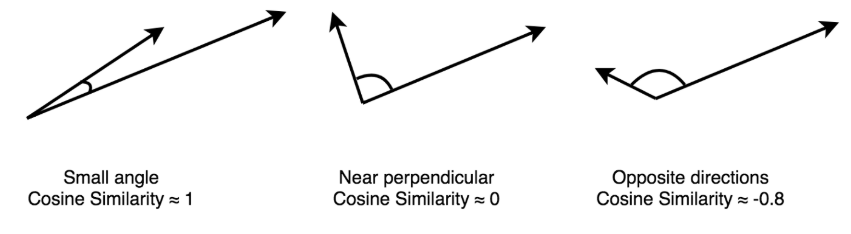
\includegraphics[width=0.7\linewidth]{cosine_similarity}
	\caption{Cosine Similarity}
	\label{fig:cosine_similarity}
\end{figure}
\noindent
Using \autoref{eq:cosine_similarity}, if we compute cosine similarity between vectors A and B, then we get:
\begin{align*}
\parallel A \parallel \parallel B \parallel &=(5 \times 3 + 0 \times 0 + 3 \times 2 + 0 \times 0 + 2 \times 2  ) = 25 \\
\parallel A \parallel  &= \sqrt{5^2 + 0^2 + 3^2 + 0^2 + 2^2}  = 6.164414 \\	     
\parallel B \parallel  &= \sqrt{3^2 + 0^2 + 2^2 + 0^2 + 2^2}  = 3.74165\\	     
sim(A,B)  &=  0.92 
\end{align*}
\noindent The value of cosine angle ranges between -1 to 1. Calculated result 0.92 shows that vector A and B are quite similar as the result inclines towards 1. As per \autoref{fig:cosine_similarity} lesser angle depicts less distance between two vectors. Hence, calculated vectors considered more similar to each other.

\subsection{Euclidean Distance Similarity}
\label{euclidean_distance}
The Euclidean distance between two points is the length between two connecting points. If we plot n-dimensional space and plot similar items, then they will fall under close proximity. Consider an example of a positive quadrant of space and we plot items on the axis which are rated by the user. The \autoref{user_movie_rating_table} illustrates the relationship between users and movies with ratings. The points are drawn on the graph in \autoref{fig:movie_plots} represents ratings given by the user to those particular movies.
\begin{table}[]
\centering
\begin{tabular}{|l|l|l|l|}
\hline
Movie/User & Lady in the water & Snakes on a plane & You Me and Dupree \\ \hline
A          & 2.5               & 3.5               & 2.5               \\ \hline
B          & 3                 & 3.5               & 3.5               \\ \hline
C          & 2.5               & 3                 &                   \\ \hline
D          &                   & 3.5               & 2.5               \\ \hline
E          & 3                 & 4                 & 2                 \\ \hline
F          & 3                 & 4                 & 3.5               \\ \hline
G          &                   & 4.5               & 1                 \\ \hline
\end{tabular}
\caption{User-Movie Rating Relationship \cite{11}}
\label{user_movie_rating_table}
\end{table}

\begin{singlespace}
\begin{figure}[H]
	\centering
	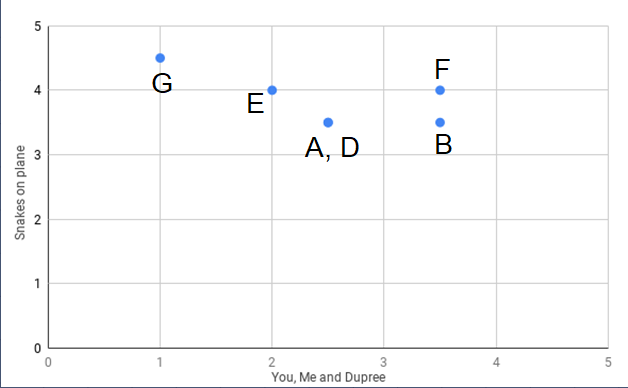
\includegraphics[width=0.7\linewidth]{movie_plots}
	\caption{Movie Rating Plots \cite{11} } 
	\label{fig:movie_plots}
\end{figure}
\end{singlespace}

\noindent In that case, we can calculate distance between items with Euclidean distance formula which is given by \autoref{euclidean_distance}. Euclidean distance is the square root of the sum of squared differences between corresponding elements of the two vectors x and y. Similarity score based on Euclidean distance can be calculated using \autoref{euclidean_simscore}. Similarity score based on euclidean's distance is defined as maximum distance divided by actual distance added to the 1. Higher distance represents lower similarity while lower distance represents higher similarity.
\\
\begin{equation}
\textrm{Euclidean Distance } = d(x,y) = \sqrt{(x_1 - y_1)^2 + ... + (x_n - y_n)^2}
\label{euclidean_distance}
\end{equation}

\begin{equation}
\textrm{Similarity score }(A,B) = \frac{1}{1+ Distance}
\label{euclidean_simscore}
\end{equation}

\noindent From above example, if we calculate Euclidean's distance between user A and user B then we get similarity score based on euclidean's distance :
\begin{align*}
Distance (A, B) &= \sqrt{(3.5 - 3.5)^{2} + (3.5 - 2.5)^{2}} \\
\textrm{Similarity score }(A,B) &= \frac{1}{1+ Distance} = 0.5
\end{align*}


\subsection{Pearson's Correlation Similarity}
\label{pearson_correlation}
Person's correlation helps in finding correlation between two users or items. Correlation values ranges from -1 to 1 \cite{20}. Correlation on higher side implies more similarity. \autoref{eq:pearson_corr} gives correlation between two users $r_{u}$ and $r_{v}$.

\begin{equation}
sim(u,v) = \frac{\sum (r_{ui} - \bar{r}_u) (r_{vi} - \bar{r}_v )}{\sqrt{(\sum (r_{ui} - \bar{r}_u))^2} \sqrt{(\sum (r_{vi} - \bar{r}_v )^2}}
\label{eq:pearson_corr}
\end{equation}

\noindent Where $r_{ui}$ and $r_{vi}$ are rating scores from two users $u$ and $v$ for an item $i$. $\bar{r}_{u}$ and $\bar{r}_{v}$ denote the average rating by the two users.
Pearson correlation score $> 0$ indicates positive association. On the other hand, Pearson correlation score $ < 0$ indicates the negative correlation and score $ = 0$ indicates no correlation. Hence a correlation value can capture a rating similarity between two users.
